{
  \centering

  \vspace*{0.2em}

  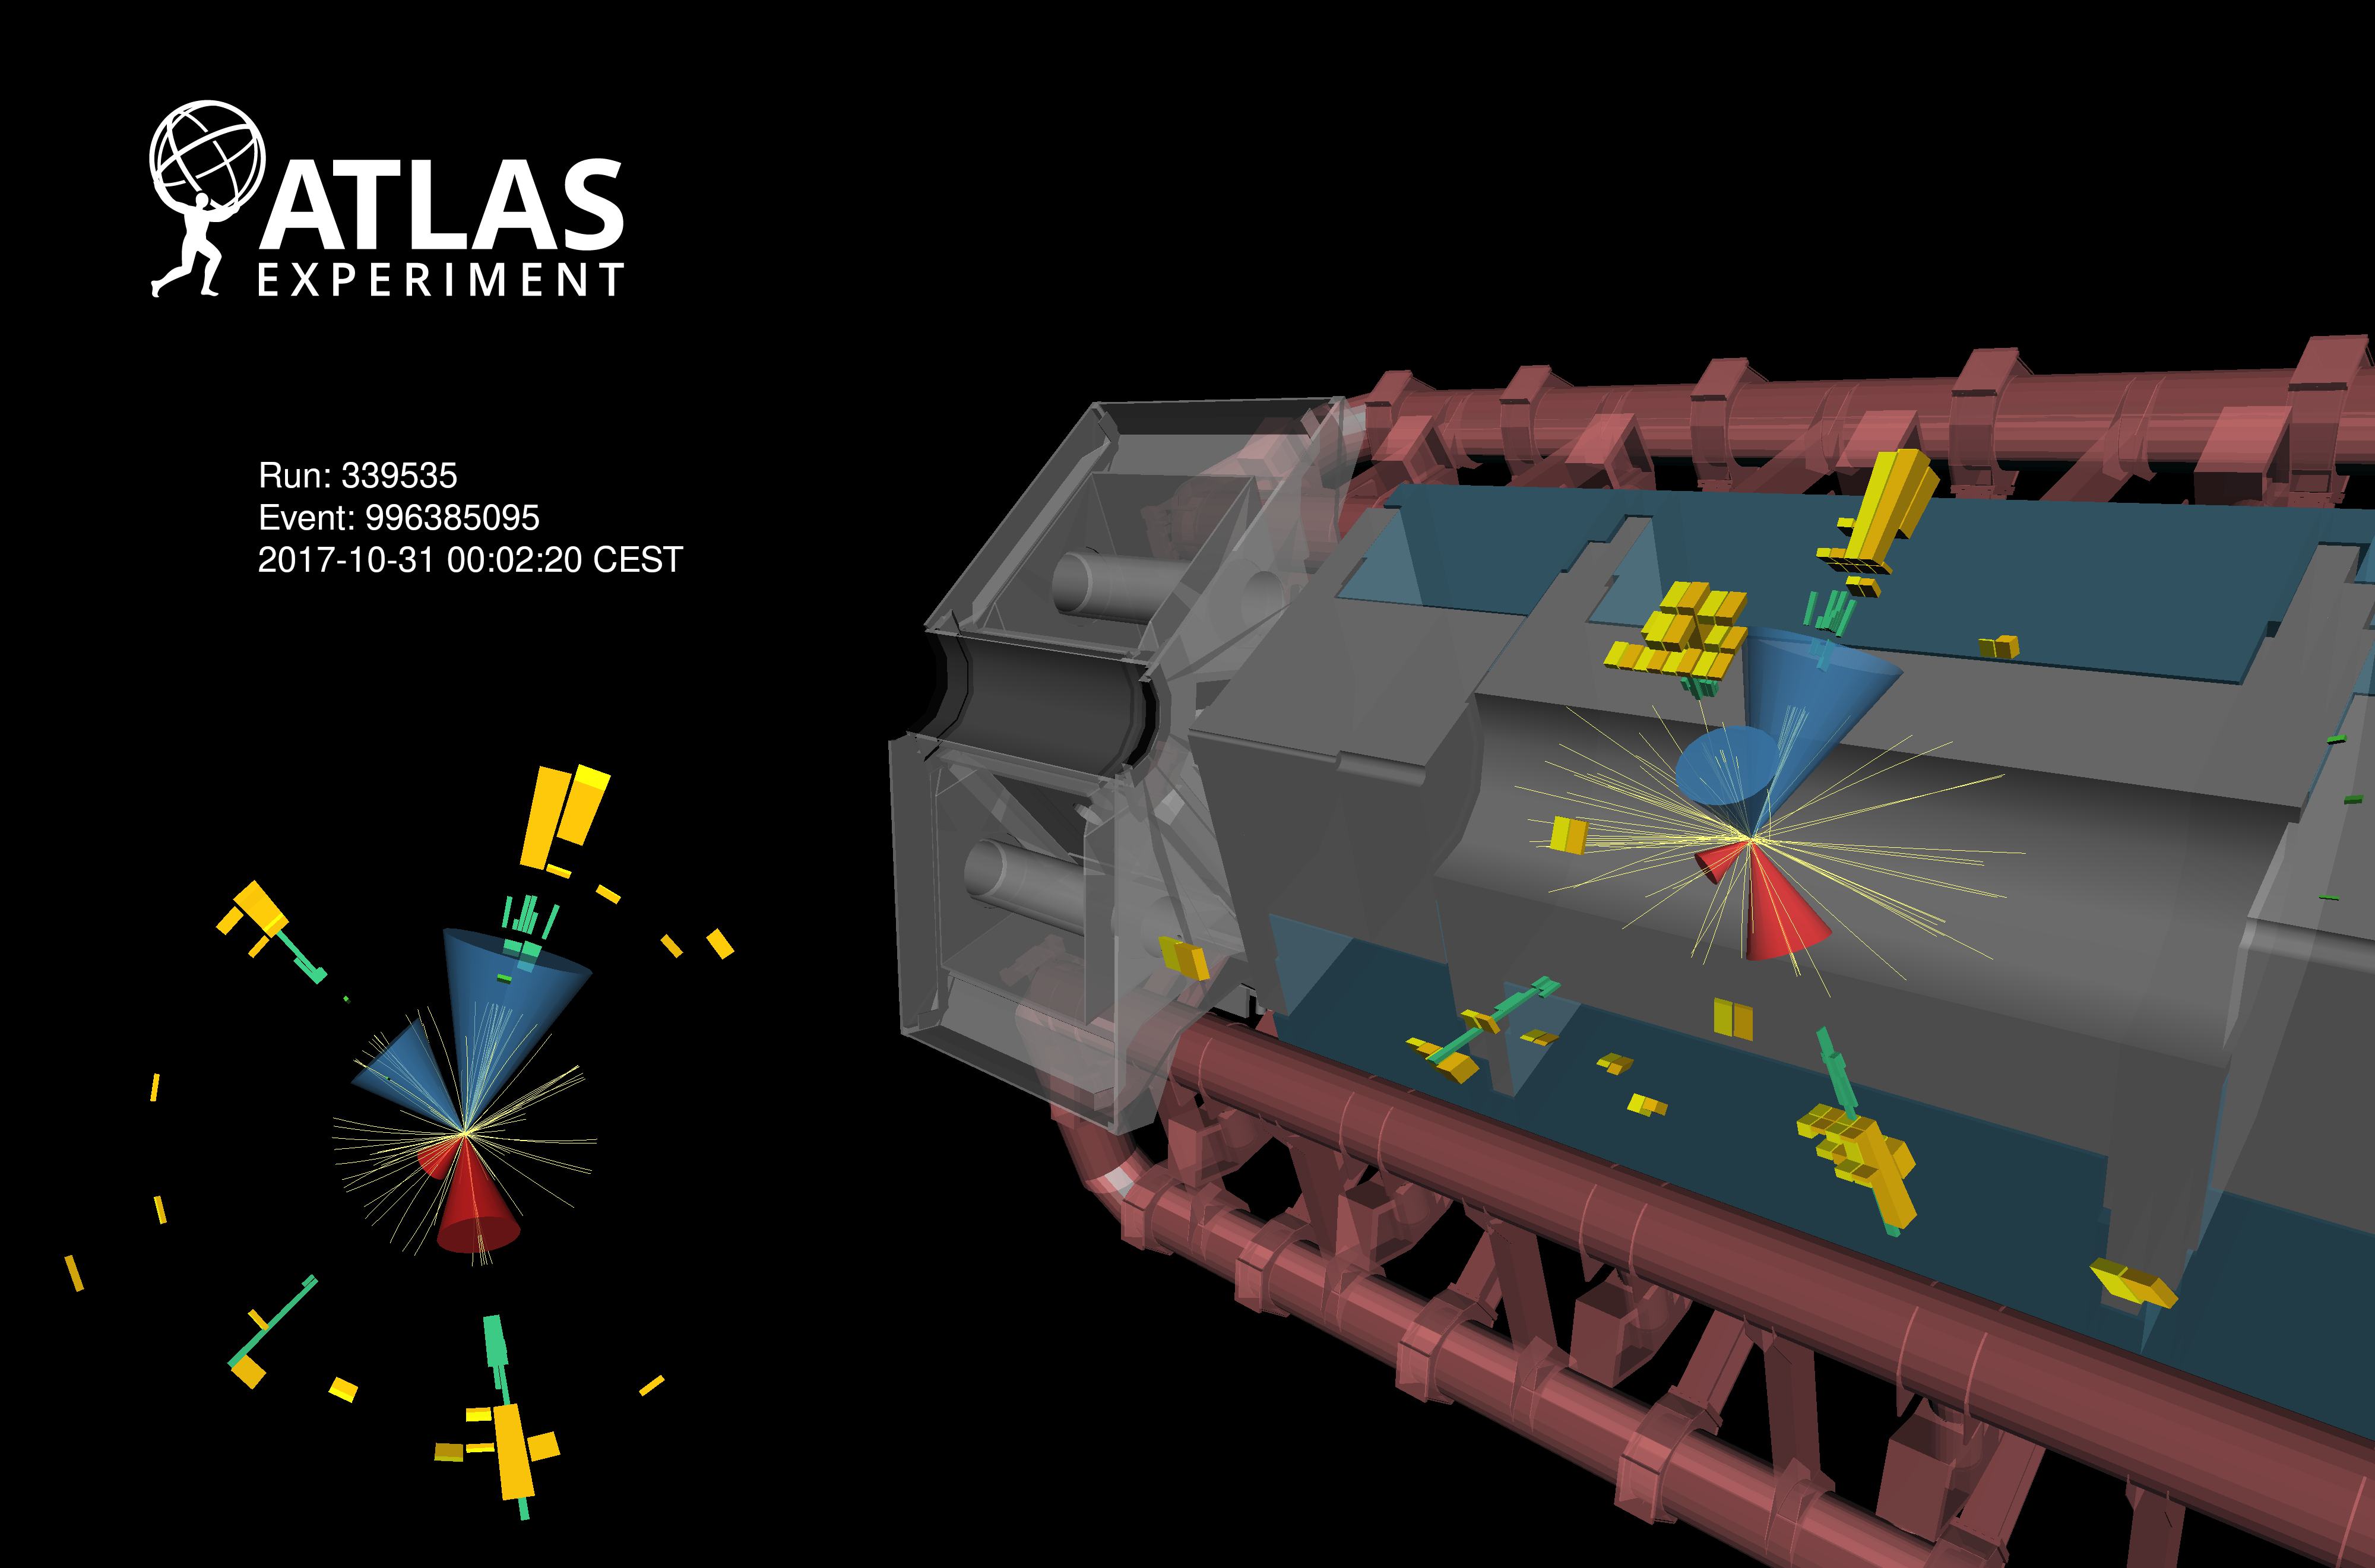
\includegraphics[width=\textwidth]{event_displays/hadhad}

  \captionof{figure}[Visualisation of the SM~\HH candidate event with the
  largest BDT score observed in data in the \hadhad channel.]{Visualisation of
    the SM~\HH candidate event with the largest BDT score observed in data in
    the \hadhad channel. The two $b$-tagged jets (blue cones) have transverse
    momenta of \SI{160}{\GeV} and \SI{100}{\GeV}. The two \tauhadvis candidates
    (red cones) have transverse momenta of \SI{100}{\GeV} and
    \SI{40}{\GeV}. Energy deposited in cells of the electromagnetic (hadronic)
    calorimeters is visualised as green (yellow) towers. Reconstructed
    charged-particle tracks are depicted as yellow lines. The event has
    $\mMMC = \SI{130}{\GeV}$, $\mBB = \SI{130}{\GeV}$, and
    $\mHH = \SI{510}{\GeV}$. The image is taken from Ref.~\cite{HDBS-2018-40}.}%
  \label{fig:event_display_hadhad}
}

{
  \centering

  \null\vfill

  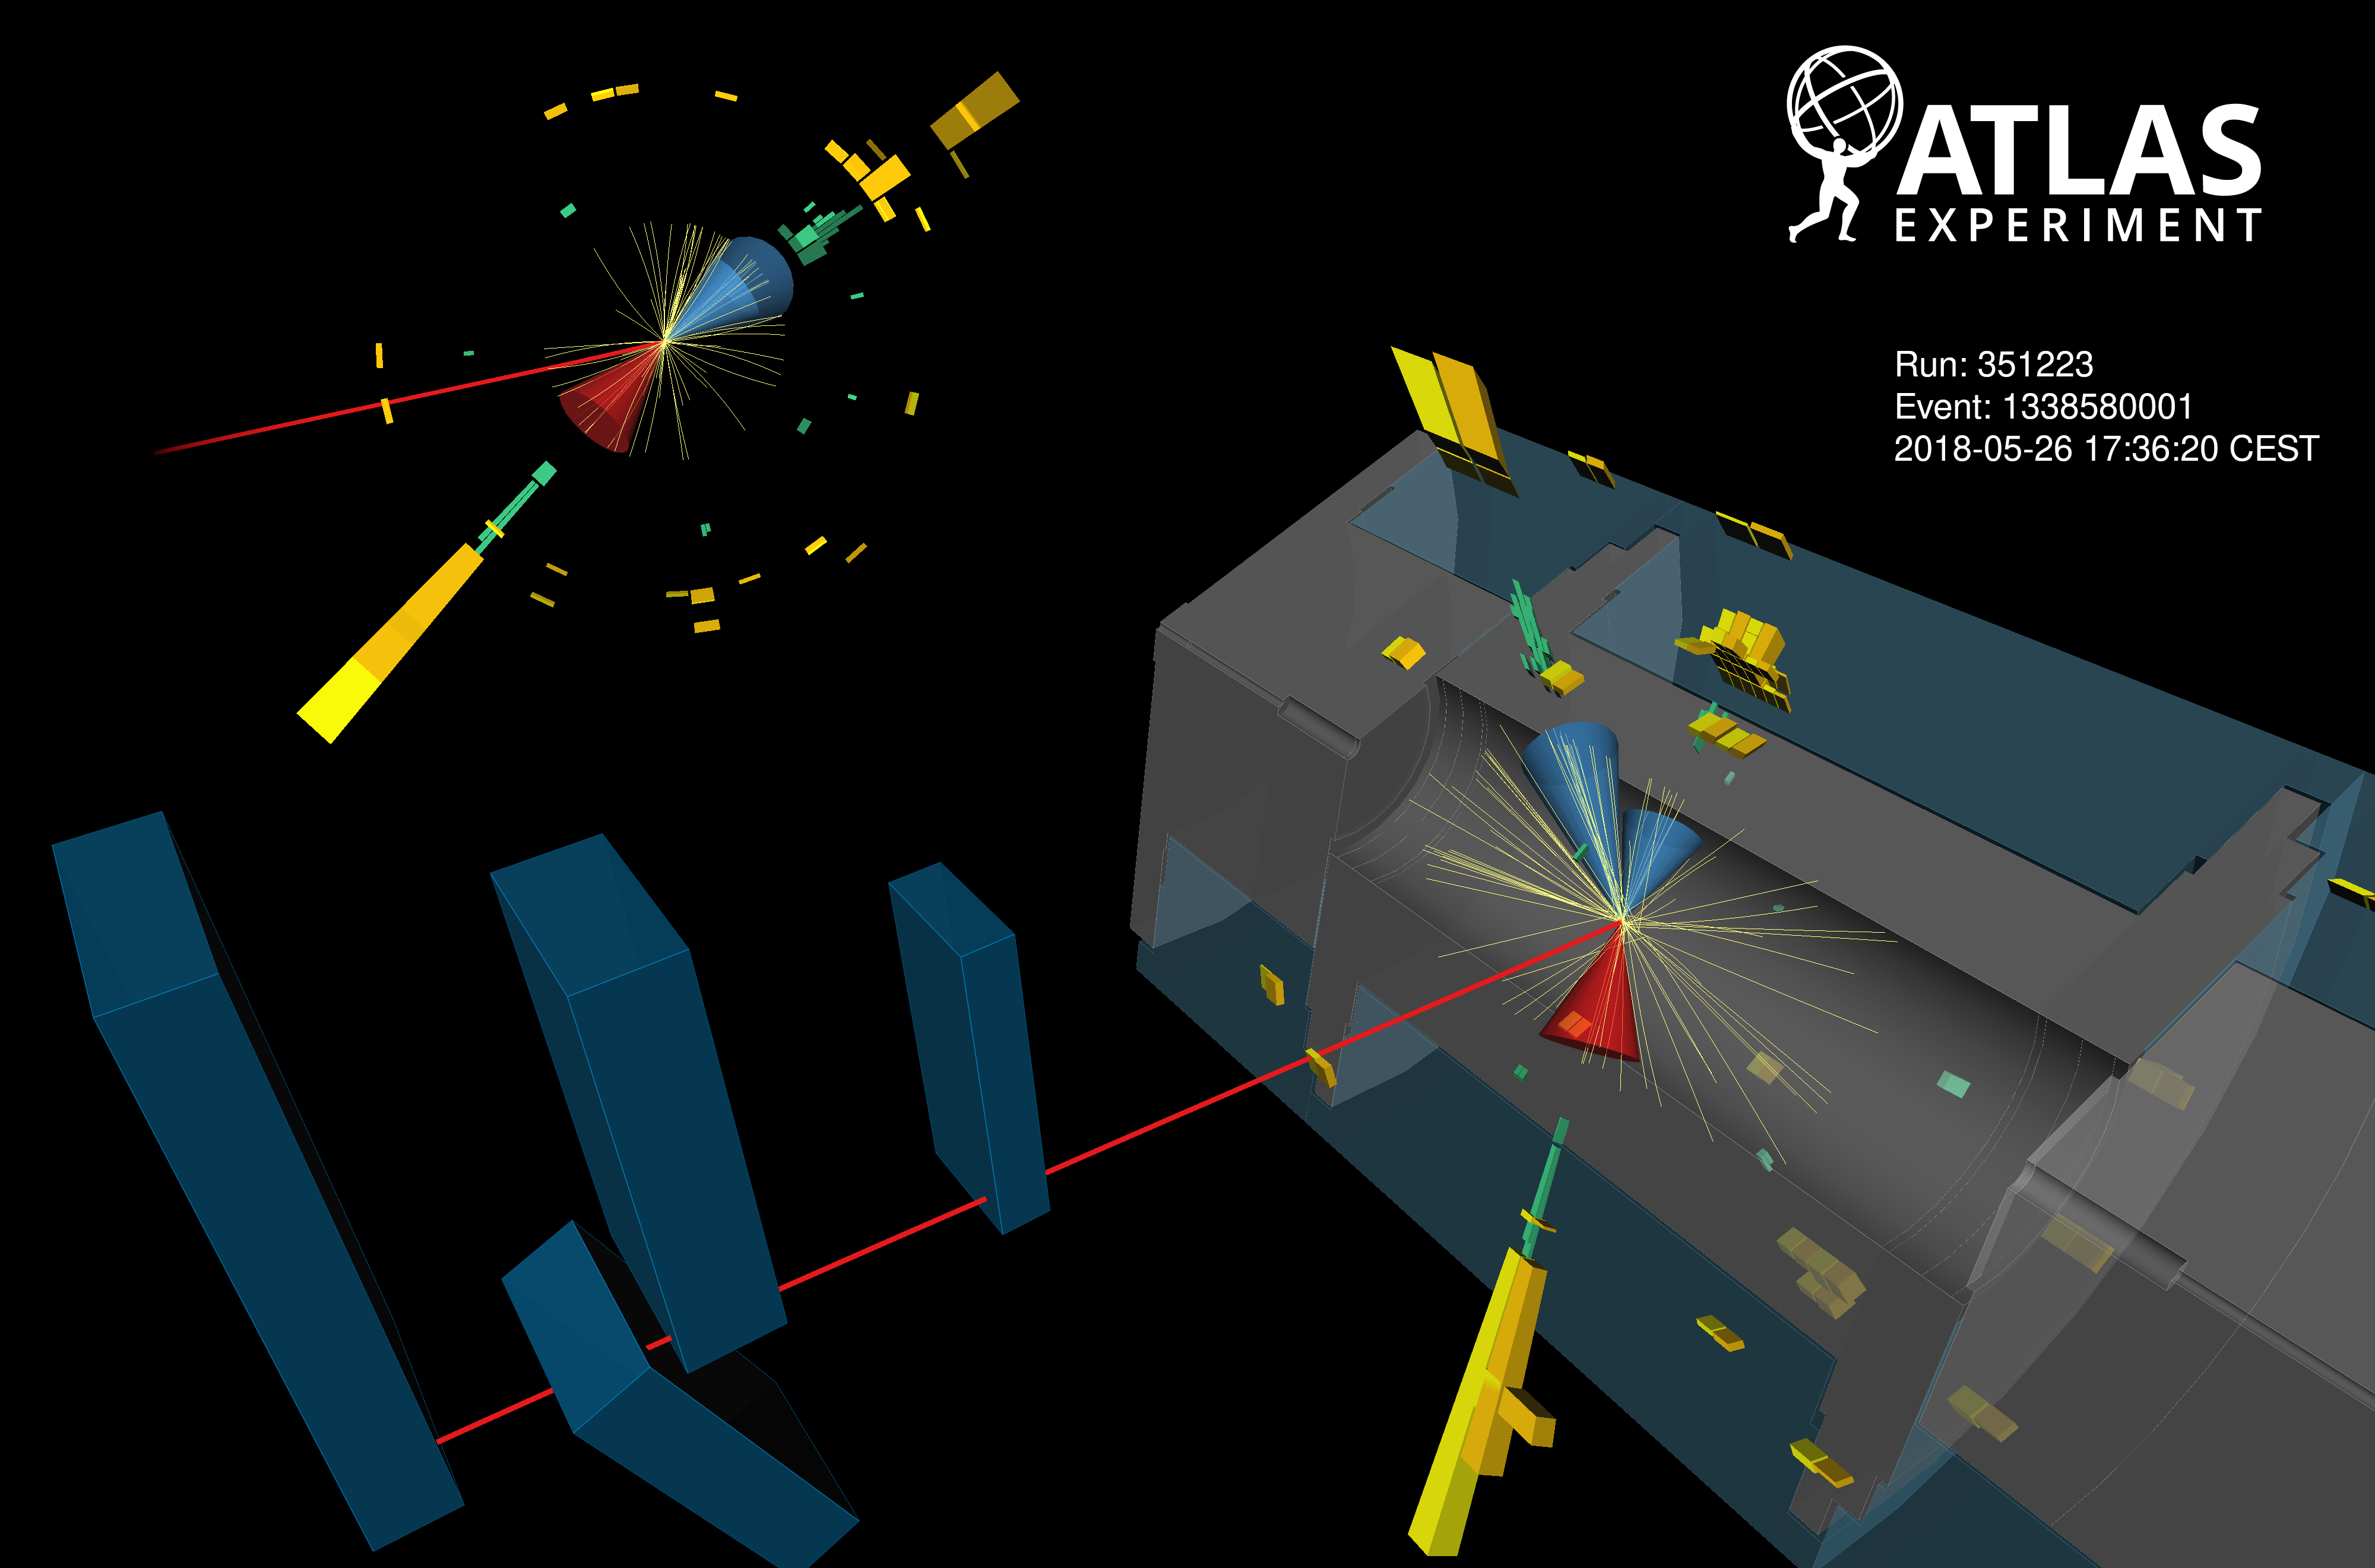
\includegraphics[width=\textwidth]{event_displays/lephad}

  \captionof{figure}[Visualisation of the SM~\HH candidate event with the
  largest NN score observed in data in the \lephad SLT channel.]{Visualisation
    of the SM~\HH candidate event with the largest NN score observed in data in
    the \lephad SLT channel. The two $b$-tagged jets (blue cones) have
    transverse momenta of \SI{190}{\GeV} and \SI{90}{\GeV}. The \tauhadvis
    candidate (red cone) has a transverse momentum of \SI{80}{\GeV}. The muon
    (red line) has a transverse momentum of \SI{30}{\GeV}. Energy deposited in
    cells of the electromagnetic (hadronic) calorimeters is visualised as green
    (yellow) towers. Reconstructed charged-particle tracks are depicted as
    yellow lines. The event has $\mMMC = \SI{120}{\GeV}$,
    $\mBB = \SI{120}{\GeV}$, and $\mHH = \SI{680}{\GeV}$. The image is taken
    from Ref.~\cite{HDBS-2018-40}.}%
  \label{fig:event_display_lephad}

  \null\vfill
}

%%% Local Variables:
%%% mode: latex
%%% TeX-master: "../../phd_thesis"
%%% End:
